\documentclass [11pt, a4wide, twoside]{article}

\usepackage{times}
\usepackage{epsfig}
\usepackage{ifthen}
\usepackage{xspace}
\usepackage{fancyhdr}
\usepackage[colorlinks,urlcolor=blue]{hyperref}
\usepackage{verbatim}
\usepackage{enumitem}
\usepackage[top=0.1mm, bottom=0.1mm, left=0.1mm, right=0.1mm]{geometry}
\usepackage{array}

\newcolumntype{C}{>{\centering\arraybackslash}m{0.12\textwidth}}
\newcolumntype{F}{>{\centering\arraybackslash}m{0.16\textwidth}}

\usepackage{listings}
\usepackage{color}

\definecolor{dkgreen}{rgb}{0,0.6,0}
\definecolor{gray}{rgb}{0.5,0.5,0.5}
\definecolor{mauve}{rgb}{0.58,0,0.82}


\graphicspath{{./figures/}}

\lstset{frame=tb,
  language=Java,
  aboveskip=0.3mm,
  belowskip=0.3mm,
  showstringspaces=false,
  columns=flexible,
  basicstyle={\small\ttfamily},
  numbers=none,
  numberstyle=\tiny\color{gray},
  keywordstyle=\color{blue},
  commentstyle=\color{dkgreen},
  stringstyle=\color{mauve},
  breaklines=true,
  breakatwhitespace=true
  tabsize=3
}


% solution switch
\newboolean{showsolution}
\setboolean{showsolution}{false} 
%\setboolean{showsolution}{false} 

\usepackage{times}
\usepackage{epsfig}
\usepackage{ifthen}
\usepackage{xspace}
\usepackage{fancyhdr}
\usepackage{amsthm}
\usepackage{hyperref}



%layout
\topmargin      -5.0mm
\oddsidemargin  6.0mm
\evensidemargin -6.0mm
\textheight     215.5mm
\textwidth      160.0mm
\parindent      1.0em
\headsep        10.3mm
\headheight     12pt
\lineskip       1pt
\normallineskip 1pt

\newtheorem{mydef}{Definition}


%header
\lhead{Software Modeling and Analysis \\ 2016}

\rhead{Prof. Oscar Nierstrasz, Mohammad Ghafari, Nevena Milojkovi\'{c} and Yuriy Tymchuk}

\lfoot{page \thepage}
\rfoot{\today}
\cfoot{}

\renewcommand{\headrulewidth}{0.1pt}
\renewcommand{\footrulewidth}{0.1pt}

%enumeration
\newenvironment{myitemize}{%
     \begin{itemize}
     \setlength{\itemsep}{0cm}}
     {\end{itemize}}

\newenvironment{myenumerate}{%
     \begin{enumerate} \setlength{\itemsep}{0cm}}
     {\end{enumerate}}


%solution
\ifthenelse{\boolean{showsolution}}
   {  \newcommand{\solution}[1]{
   	\noindent\underline{\textbf{Answer:}}\\[2mm]
   	 \textsl{#1}
	 \vspace{10pt}
	 \normalsize
	}
  }
  {  \newcommand{\solution}[1]{} }


\pagestyle{fancy}

% ============================================================
% Markup macros for proof-reading
\usepackage{ifthen}
\usepackage[normalem]{ulem} % for \sout
\usepackage{xcolor}
\newcommand{\ra}{$\rightarrow$}
\newboolean{showedits}
\setboolean{showedits}{true} % toggle to show or hide edits
\ifthenelse{\boolean{showedits}}
{
	\newcommand{\ugh}[1]{\textcolor{red}{\uwave{#1}}} % please rephrase
	\newcommand{\ins}[1]{\textcolor{blue}{\uline{#1}}} % please insert
	\newcommand{\del}[1]{\textcolor{red}{\sout{#1}}} % please delete
	\newcommand{\chg}[2]{\textcolor{red}{\sout{#1}}{\ra}\textcolor{blue}{\uline{#2}}} % please change
}{
	\newcommand{\ugh}[1]{#1} % please rephrase
	\newcommand{\ins}[1]{#1} % please insert
	\newcommand{\del}[1]{} % please delete
	\newcommand{\chg}[2]{#2}
}
% ============================================================
% Put edit comments in a really ugly standout display
%\usepackage{ifthen}
\usepackage{amssymb}
\newboolean{showcomments}
\setboolean{showcomments}{true}
%\setboolean{showcomments}{false}
\newcommand{\id}[1]{$-$Id: scgPaper.tex 32478 2010-04-29 09:11:32Z oscar $-$}
\newcommand{\yellowbox}[1]{\fcolorbox{gray}{yellow}{\bfseries\sffamily\scriptsize#1}}
\newcommand{\triangles}[1]{{\sf\small$\blacktriangleright$\textit{#1}$\blacktriangleleft$}}
\ifthenelse{\boolean{showcomments}}
%{\newcommand{\nb}[2]{{\yellowbox{#1}\triangles{#2}}}
{\newcommand{\nbc}[3]{
 {\colorbox{#3}{\bfseries\sffamily\scriptsize\textcolor{white}{#1}}}
 {\textcolor{#3}{\sf\small$\blacktriangleright$\textit{#2}$\blacktriangleleft$}}}
 \newcommand{\version}{\emph{\scriptsize\id}}}
{\newcommand{\nbc}[3]{}
 \renewcommand{\ugh}[1]{#1} % please rephrase
 \renewcommand{\ins}[1]{#1} % please insert
 \renewcommand{\del}[1]{} % please delete
 \renewcommand{\chg}[2]{#2} % please change
 \newcommand{\version}{}}
\newcommand{\nb}[2]{\nbc{#1}{#2}{orange}}
\newcommand{\here}{\yellowbox{$\Rightarrow$ CONTINUE HERE $\Leftarrow$}}
\newcommand\rev[2]{\nb{TODO (rev #1)}{#2}} % reviewer comments
\newcommand\fix[1]{\nb{FIX}{#1}}
\newcommand\todo[1]{\nb{TO DO}{#1}}
\newcommand\on[1]{\nbc{ON}{#1}{red}} % add more author macros here
%\newcommand\XXX[1]{\nbc{XXX}{#1}{blue}}
%\newcommand\XXX[1]{\nbc{XXX}{#1}{brown}}
%\newcommand\XXX[1]{\nbc{XXX}{#1}{cyan}}
%\newcommand\XXX[1]{\nbc{XXX}{#1}{darkgray}}
%\newcommand\XXX[1]{\nbc{XXX}{#1}{gray}}
%\newcommand\XXX[1]{\nbc{XXX}{#1}{magenta}}
%\newcommand\XXX[1]{\nbc{XXX}{#1}{olive}}
%\newcommand\XXX[1]{\nbc{XXX}{#1}{orange}}
%\newcommand\XXX[1]{\nbc{XXX}{#1}{purple}}
%\newcommand\XXX[1]{\nbc{XXX}{#1}{red}}
%\newcommand\XXX[1]{\nbc{XXX}{#1}{teal}}
%\newcommand\XXX[1]{\nbc{XXX}{#1}{violet}}
%=============================================================
% ST80 listings macros
% Adapted from Squeak by Example book
%=============================================================
% If you want >>> appearing as right guillemet, you need these two lines:
%\usepackage[T1]{fontenc}
%\newcommand{\sep}{\mbox{>>}}
% Otherwise use this:
\newcommand{\sep}{\mbox{$\gg$}}
%=============================================================
%:\needlines{N} before code block to force page feed
\usepackage{needspace}
\newcommand{\needlines}[1]{\Needspace{#1\baselineskip}}
%=============================================================
%:Listings package configuration for ST80
\usepackage[english]{babel}
\usepackage{amssymb,textcomp}
\usepackage{listings}
% \usepackage[usenames,dvipsnames]{color}
% \usepackage[usenames]{color}
% \definecolor{source}{gray}{0.95}
\lstdefinelanguage{Smalltalk}{
%  morekeywords={self,super,true,false,nil,thisContext}, % This is overkill
  morestring=[d]',
  morecomment=[s]{"}{"},
  alsoletter={\#:},
  escapechar={!},
  literate=
    {BANG}{!}1
    {UNDERSCORE}{\_}1
    {\\st}{Smalltalk}9 % convenience -- in case \st occurs in code
    % {'}{{\textquotesingle}}1 % replaced by upquote=true in \lstset
    {_}{{$\leftarrow$}}1
    {>>>}{{\sep}}1
    {^}{{$\uparrow$}}1
    {~}{{$\sim$}}1
    {-}{{\sf -\hspace{-0.13em}-}}1  % the goal is to make - the same width as +
    {+}{\raisebox{0.08ex}{+}}1		% and to raise + off the baseline to match -
    {-->}{{\quad$\longrightarrow$\quad}}3
	, % Don't forget the comma at the end!
  tabsize=4
}[keywords,comments,strings]

\definecolor{source}{gray}{0.95}

\lstset{language=Smalltalk,
	basicstyle=\sffamily,
	keywordstyle=\color{black}\bfseries,
	% stringstyle=\ttfamily, % Ugly! do we really want this? -- on
	mathescape=true,
	showstringspaces=false,
	keepspaces=true,
	breaklines=true,
	breakautoindent=true,
	backgroundcolor=\color{source},
	lineskip={-1pt}, % Ugly hack
	upquote=true, % straight quote; requires textcomp package
	columns=fullflexible} % no fixed width fonts
% In-line code (literal)
% Normally use this for all in-line code:
\newcommand{\ct}{\lstinline[mathescape=false,backgroundcolor=\color{white},basicstyle={\sffamily\upshape}]}
% In-line code (latex enabled)
% Use this only in special situations where \ct does not work
% (within section headings ...):
\newcommand{\lct}[1]{{\textsf{\textup{#1}}}}
% Code environments
\lstnewenvironment{code}{%
	\lstset{%
		% frame=lines,
		frame=single,
		framerule=0pt,
		mathescape=false
	}
}{}

% Useful to add a matching $ after code containing a $
% \def\ignoredollar#1{}
%=============================================================
\newcommand{\ie}{\emph{i.e.}\xspace}
\newcommand{\eg}{\emph{e.g.}\xspace}
\newcommand{\etal}{\emph{et al.}\xspace}
% ============================================================


\begin{document}

% title
\section*{\ifthenelse{\boolean{showsolution}}{Solution }{}Final Exam, 21. 12. 2016.}

% - - - - - - - - - - - - - - - - - - - - - - - - - - - - - - - - - - - - - - - - - - - - - - - - - - - - - - - - - - - - - - - - - - -
\subsection*{Name: \\ Immatriculation number:}

\subsection*{Exercise 1}
What is the difference between reflection and reification? 
\vspace{4cm}

\subsection*{Exercise 2}
What is the difference between an instance variable, a class variable and an instance variable on the class side in Smalltalk?

\vspace{4cm}

\subsection*{Exercise 3}
What is the difference between \lct{CallGraph} and \lct{CallGraph class}? What is the result of the execution of code snippet \lct{Object newAnonymousSubclass class} in Pharo?
\vspace{4cm}

\newpage

\subsection*{Exercise 4}
What is similar and what is different between \lct{self} and \lct{super} in Smalltalk?
\vspace{4cm}

\subsection*{Exercise 5}
How would you intercept every invocation of the method \ct{String>>>#,} in Smalltalk so it would print the concatenation result to the \ct{Transcript}? For example, the following code should print " Modeling Analysis Exam" to the \ct{Transcript}.
\begin{lstlisting}
title := 'Software', ' Modeling', ' Analysis'.
title := title substrings collect: #first.
title := title joinUsing: ''.
title := title, ' Exam'
\end{lstlisting}
\vspace{4cm}

\subsection*{Exercise 6}
What are the Data Classes and how does the Data Class detection strategy work?
\vspace{4cm}



\subsection*{Name: \\ Immatriculation number:}

\subsection*{Exercise 7}
The following polymetric view visualizes a part of the Argo UML project. Classes are represented by rectangles, and inheritance is represented by the edges between classes with subclasses positioned below their superclass. The width of the rectangles represents the number of attributes of a class, height corresponds to the number of methods, and the rectangles with a darker fill color represent classes with a higher number of lines of code. Look at the diagram and derive some most outstanding features/anti-patterns about the hierarchies \textbf{A}, and \textbf{B} and the classes \textbf{C}, and \textbf{D}.

\begin{figure}[h!]
  \centering
  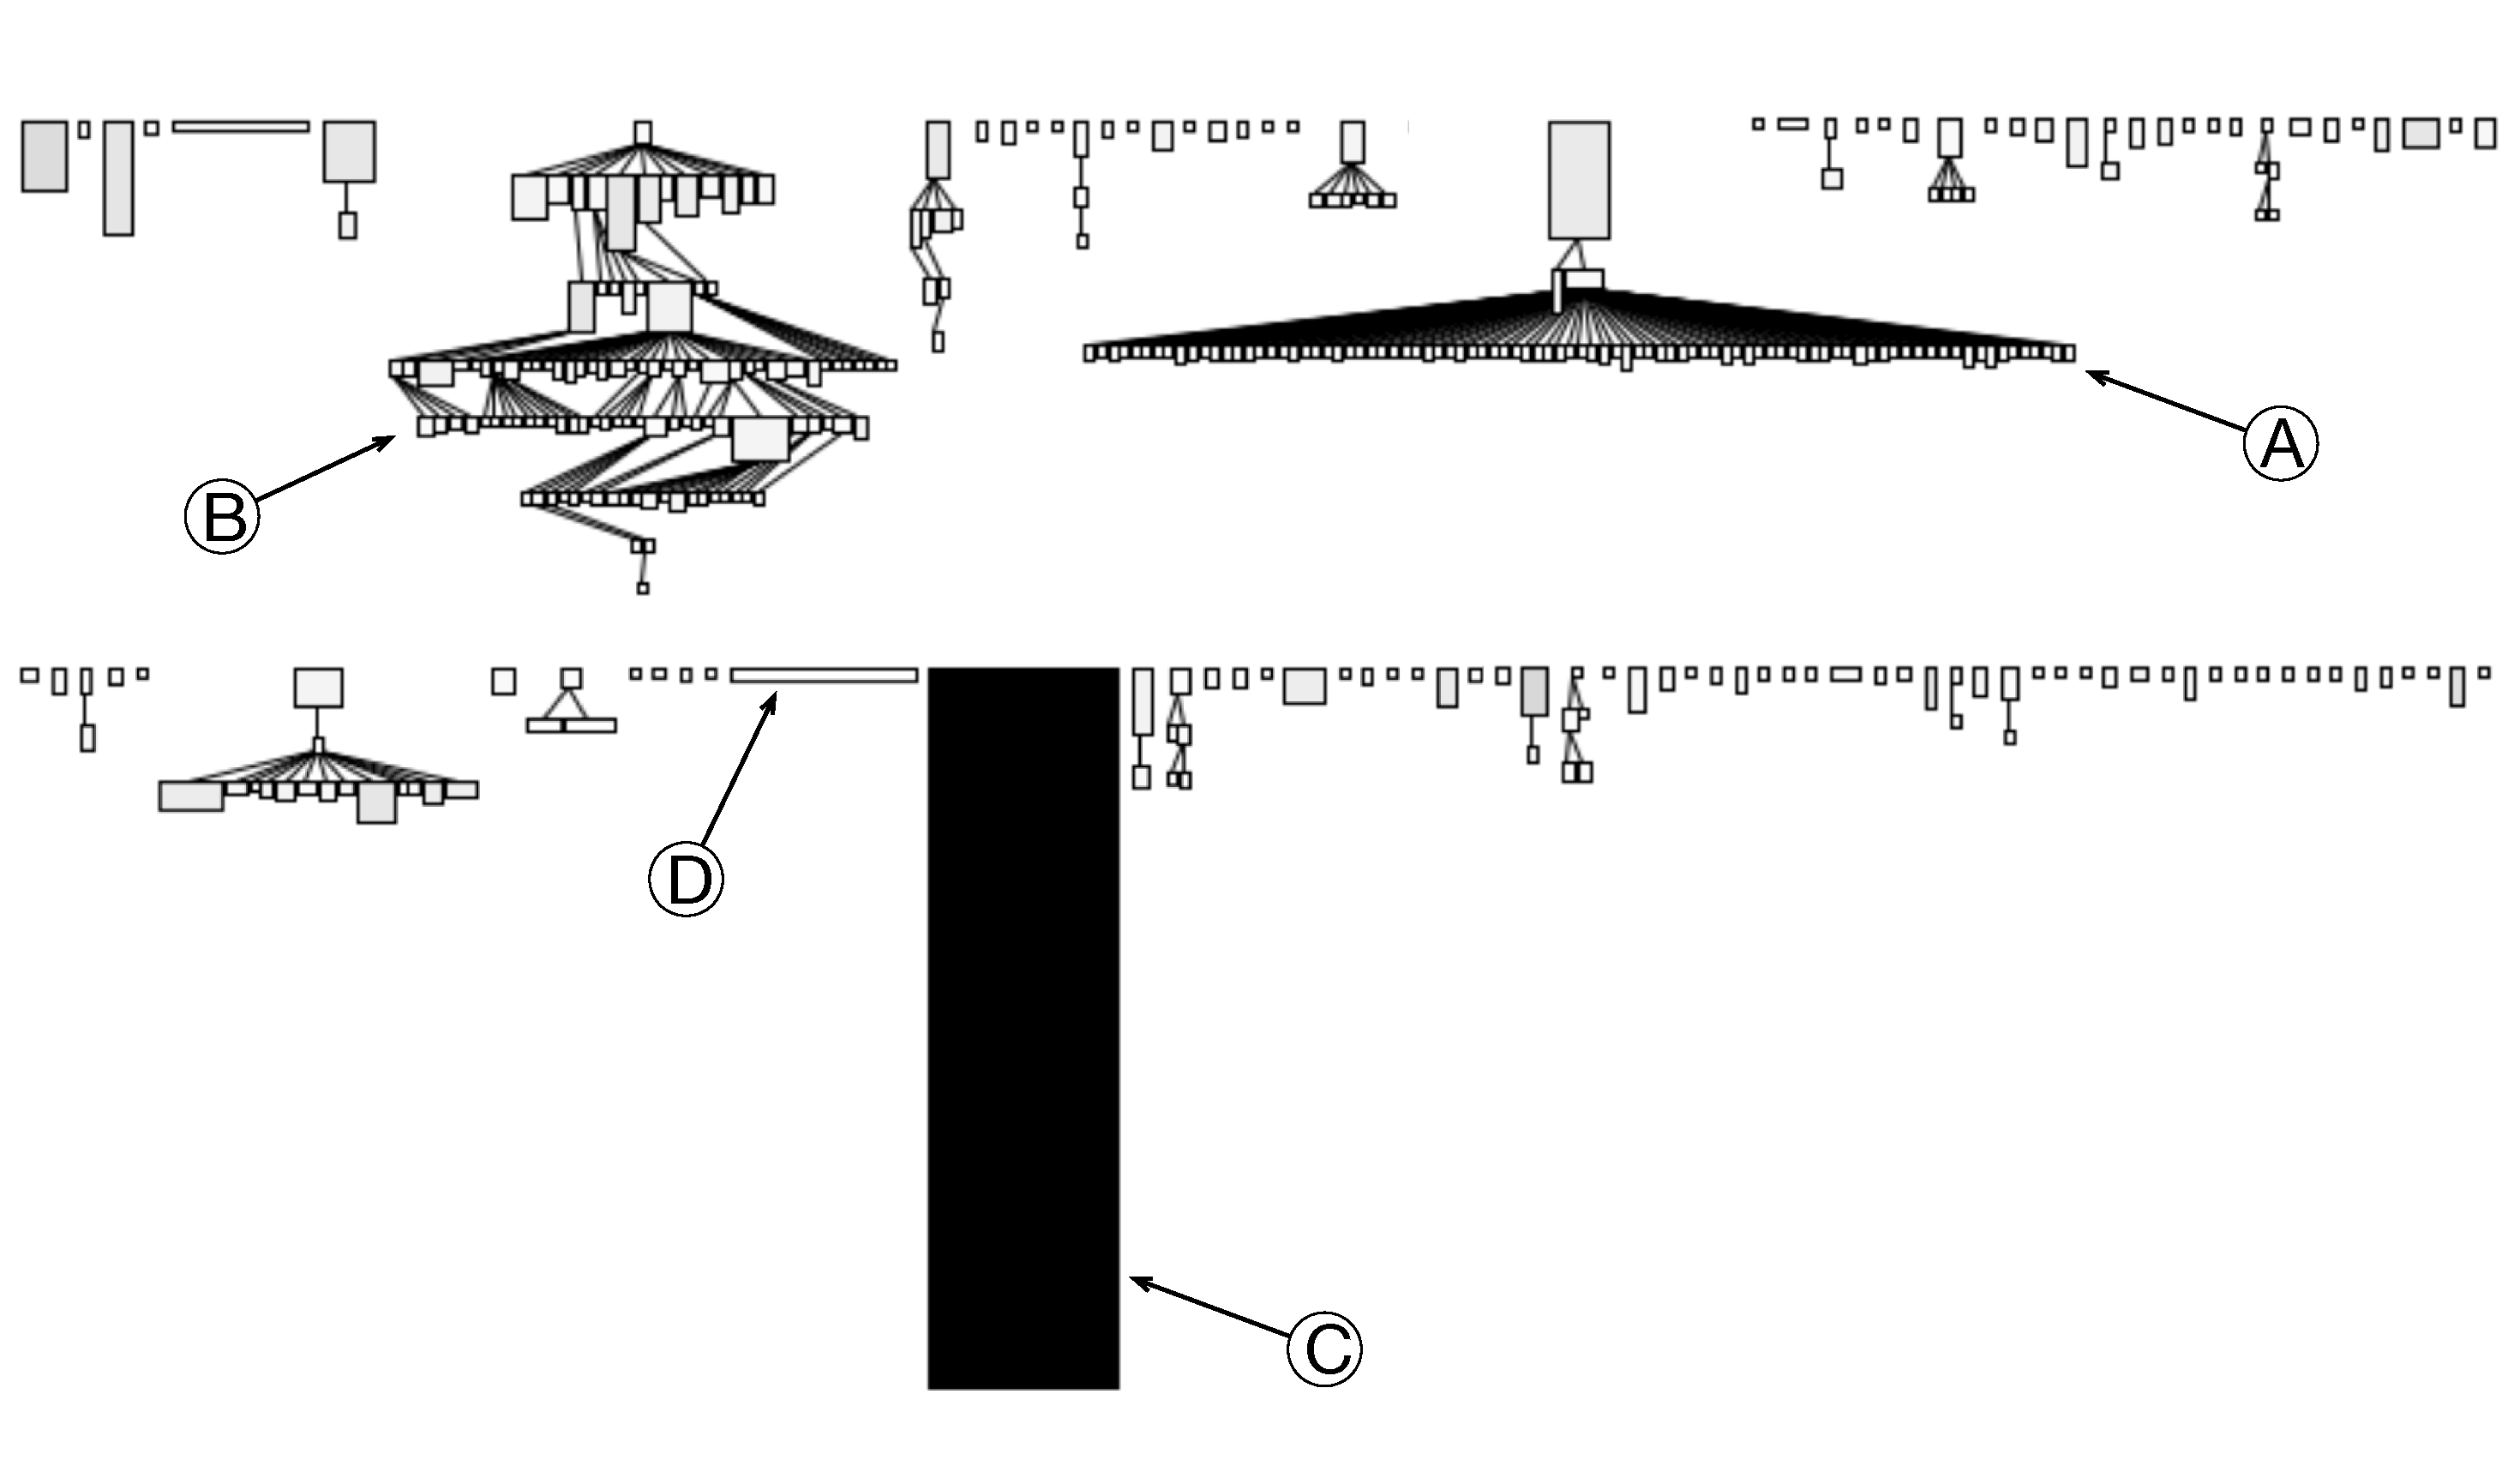
\includegraphics[width=0.9\textwidth]{argo-viz}
\end{figure}
\begin{enumerate}[label=(\Alph*)]
\item 
\item \vspace{1cm}
\item \vspace{1cm}
\item \vspace{1cm}
\end{enumerate}
\vspace{1cm}

\subsection*{Exercise 8}
What is the difference between coupling and cohesion?
\vspace{4cm}

\subsection*{Exercise 9}
What is the relation between source code change metrics and bugs in the software system?
\vspace{4cm}

\subsection*{Exercise 10}
How can dynamic analysis be performed? What are the limitations of static analysis?
\vspace{4cm}

\newpage
\subsection*{Name: \\ Immatriculation number:}
\subsection*{Exercise 11}
Imagine that the boss of your software company wants to add code review to the development workflow of your team and asks you to look up the available tools. You found Microsoft's CodeFlow, Collaborator of SmartBear, Facebook's Differential, and Gerrit developed by Google. You assemble the following table with the features of these tools:

\begin{table}[h]
\centering
\begin{tabular}{lCCCFC}
             & Diff for Images & Grouping of Reviewers & Review Watchers & Commenting on any Selection  & OSS License \\ \hline
CodeFlow     & \textbf{}       & \textbf{}             & \textbf{}       & \textbf{X}                   & \textbf{}   \\ \hline
Collaborator & \textbf{X}      & \textbf{X}            & \textbf{X}      & \textbf{}                    & \textbf{}   \\ \hline
Differential & \textbf{}       & \textbf{}             & \textbf{X}      & \textbf{}                    & \textbf{X}  \\ \hline
Gerrit       & \textbf{X}      & \textbf{}             & \textbf{X}      & \textbf{X}                   & \textbf{X}  \\ \hline
\end{tabular}
\end{table}

To have a good overview of all the tools and their features, you have to draw a concept lattice. Also your boss likes to be aware of everything that is happening and to put her two cents in technical questions. That's why she wants a tool that supports \emph{Review Watchers} and \emph{Commenting on any Selection}. If there is a tool that has both features, she will be interested to know what other features it has. This is why you have to compute the closure of \{Review Watchers, Commenting on any Selection\}



\end{document}
